\documentclass[a4paper, 12pt]{article}

\usepackage{cmap}
\usepackage[OT1]{fontenc}
\usepackage[utf8]{inputenc}
%\usepackage{mathtext}
%\usepackage{amsmath}
\usepackage[russian]{babel}
\usepackage{amsmath}
\usepackage{amsfonts}
\usepackage{amssymb}
\usepackage{graphicx}
%\usepackage[bookmarks=true, pdfpagemode=UseNone]{hyperref}
\usepackage{indentfirst}
\usepackage{listings}
%\usepackage{multicol}
%\usepackage{misccorr}
%\usepackage{longtable}
%\usepackage{flafter}
\usepackage{float}
%\usepackage{color}
%\usepackage{nccfloats}
%\usepackage{tabularx}
%\usepackage{graphicx}
%\usepackage[babel=true,protrusion=true,expansion=true]{microtype}
%\usepackage[left=1.8cm, right=1cm, top=1cm, bottom=1cm, bindingoffset=0cm]{geometry}

%\pagestyle{empty}

\author{Алексюк А.О., Мурашко Д.С.}
\title{Визуализация сигналов во временной и частотной области}
\lstset{inputencoding=utf8, extendedchars=\true, keepspaces = true, language=Matlab}

\begin{document}
\maketitle
\tableofcontents
\pagebreak

\begin{lstlisting}
x = 0:0.01:4*pi;
f0 = 5;
%исходный сигнал
y = sin(2*pi*f0*x);
plot(x(1:200),y(1:200))
grid
%спектр исходного сигнала
figure
spectrum = fft(y,512);
norm_spectrum = spectrum.*conj(spectrum)/512;
f=100*(0:255)/512;
plot(f, norm_spectrum(1:256))
axis([0 max(f) 0 10])
grid
\end{lstlisting}

\begin{figure}[H]
   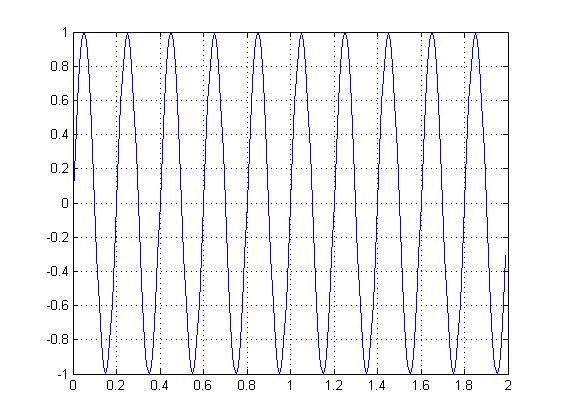
\includegraphics[width=\textwidth]{sin.png}
   \caption{Синусоида}
\end{figure}

\begin{figure}[H]
   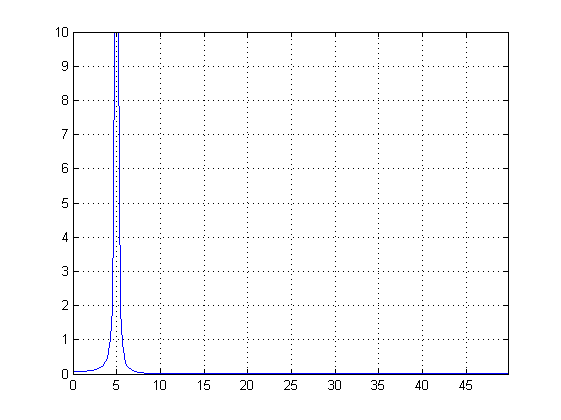
\includegraphics[width=\textwidth]{spectre.png}
   \caption{Спектр}
\end{figure}

\end{document}